%\documentclass[12pt]{article}
%\usepackage[a4paper, margin=1in]{geometry} 
%\usepackage{graphicx} 
%\usepackage{hyperref}
%\usepackage{float}
%\usepackage{multicol}
%\usepackage{amsmath}
%\usepackage[ruled]{algorithm2e}
%\usepackage{amssymb}
%\usepackage[font=small, labelfont=bf]{caption}
%
%\begin{document}

%
% Dot matrix
%
\subsection{Dot matrix}
Using a dot matrix is an effective and easy way to find local similarities.

%
% Basic concept
%
\subsubsection*{Basic concept}
It uses an $m \times n$ binary matrix from two sequences.

\begin{itemize}
\item A dot: match
\item Empty: mismatch
\end{itemize}

%
% Example of dot matrix
%
\subsubsection*{Example of dot matrix}
\begin{verbatim}
    q: ACATTAG, d: CATTTAGG
\end{verbatim}

\begin{figure}[H]
  \centering
      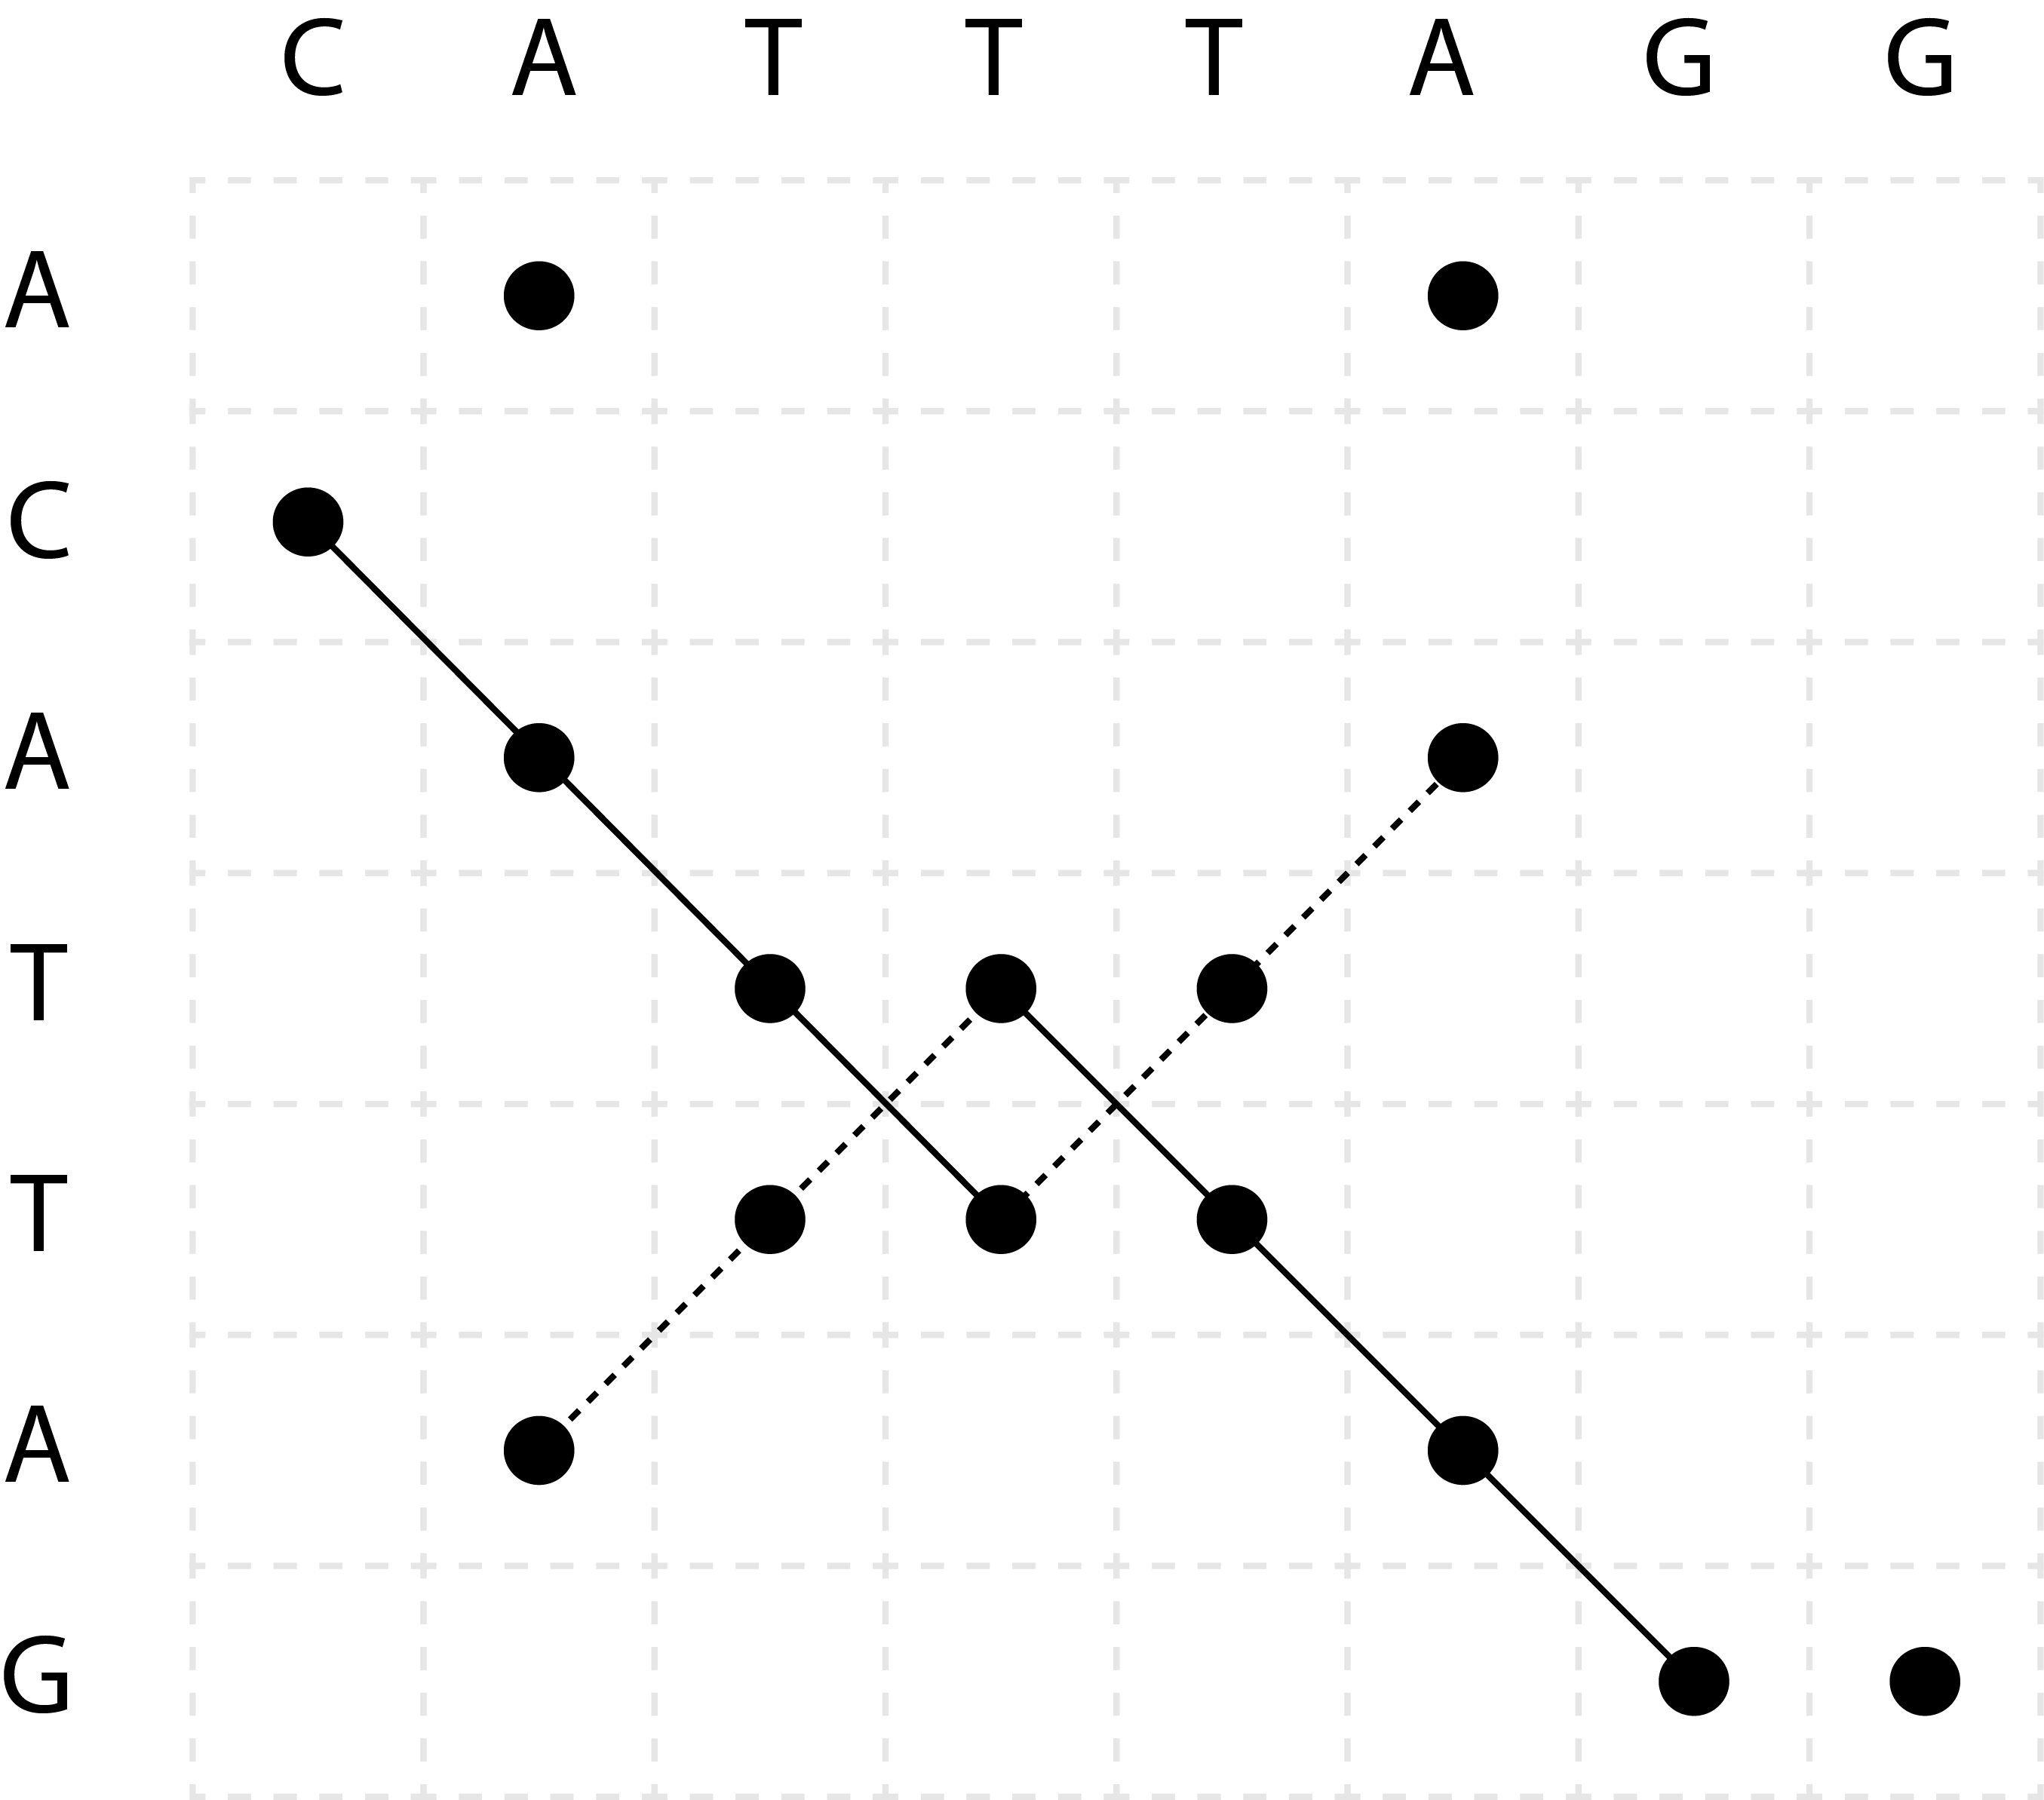
\includegraphics[width=0.3\textwidth]{fig04/dot_matrix.png}
  \caption{Dot matrix of $7 \times 8$}
\end{figure}

\noindent
It is easy to find segment pairs with a dot matrix. Contiguous dots along diagonals indicate local alignments. It is also easy to find other similarities. For instance, contiguous dots along anti-diagonals indicate reversed substrings.

%
% Filtering of dot matrix
%
\subsubsection*{Filtering of dot matrix}
Dot matrices usually get noisy with too many dots.  Overlapping windows are usually applied to reduce the noise.

\bigskip 
\noindent
\textbf{Example of filtering}

\begin{figure}[H]
  \centering
      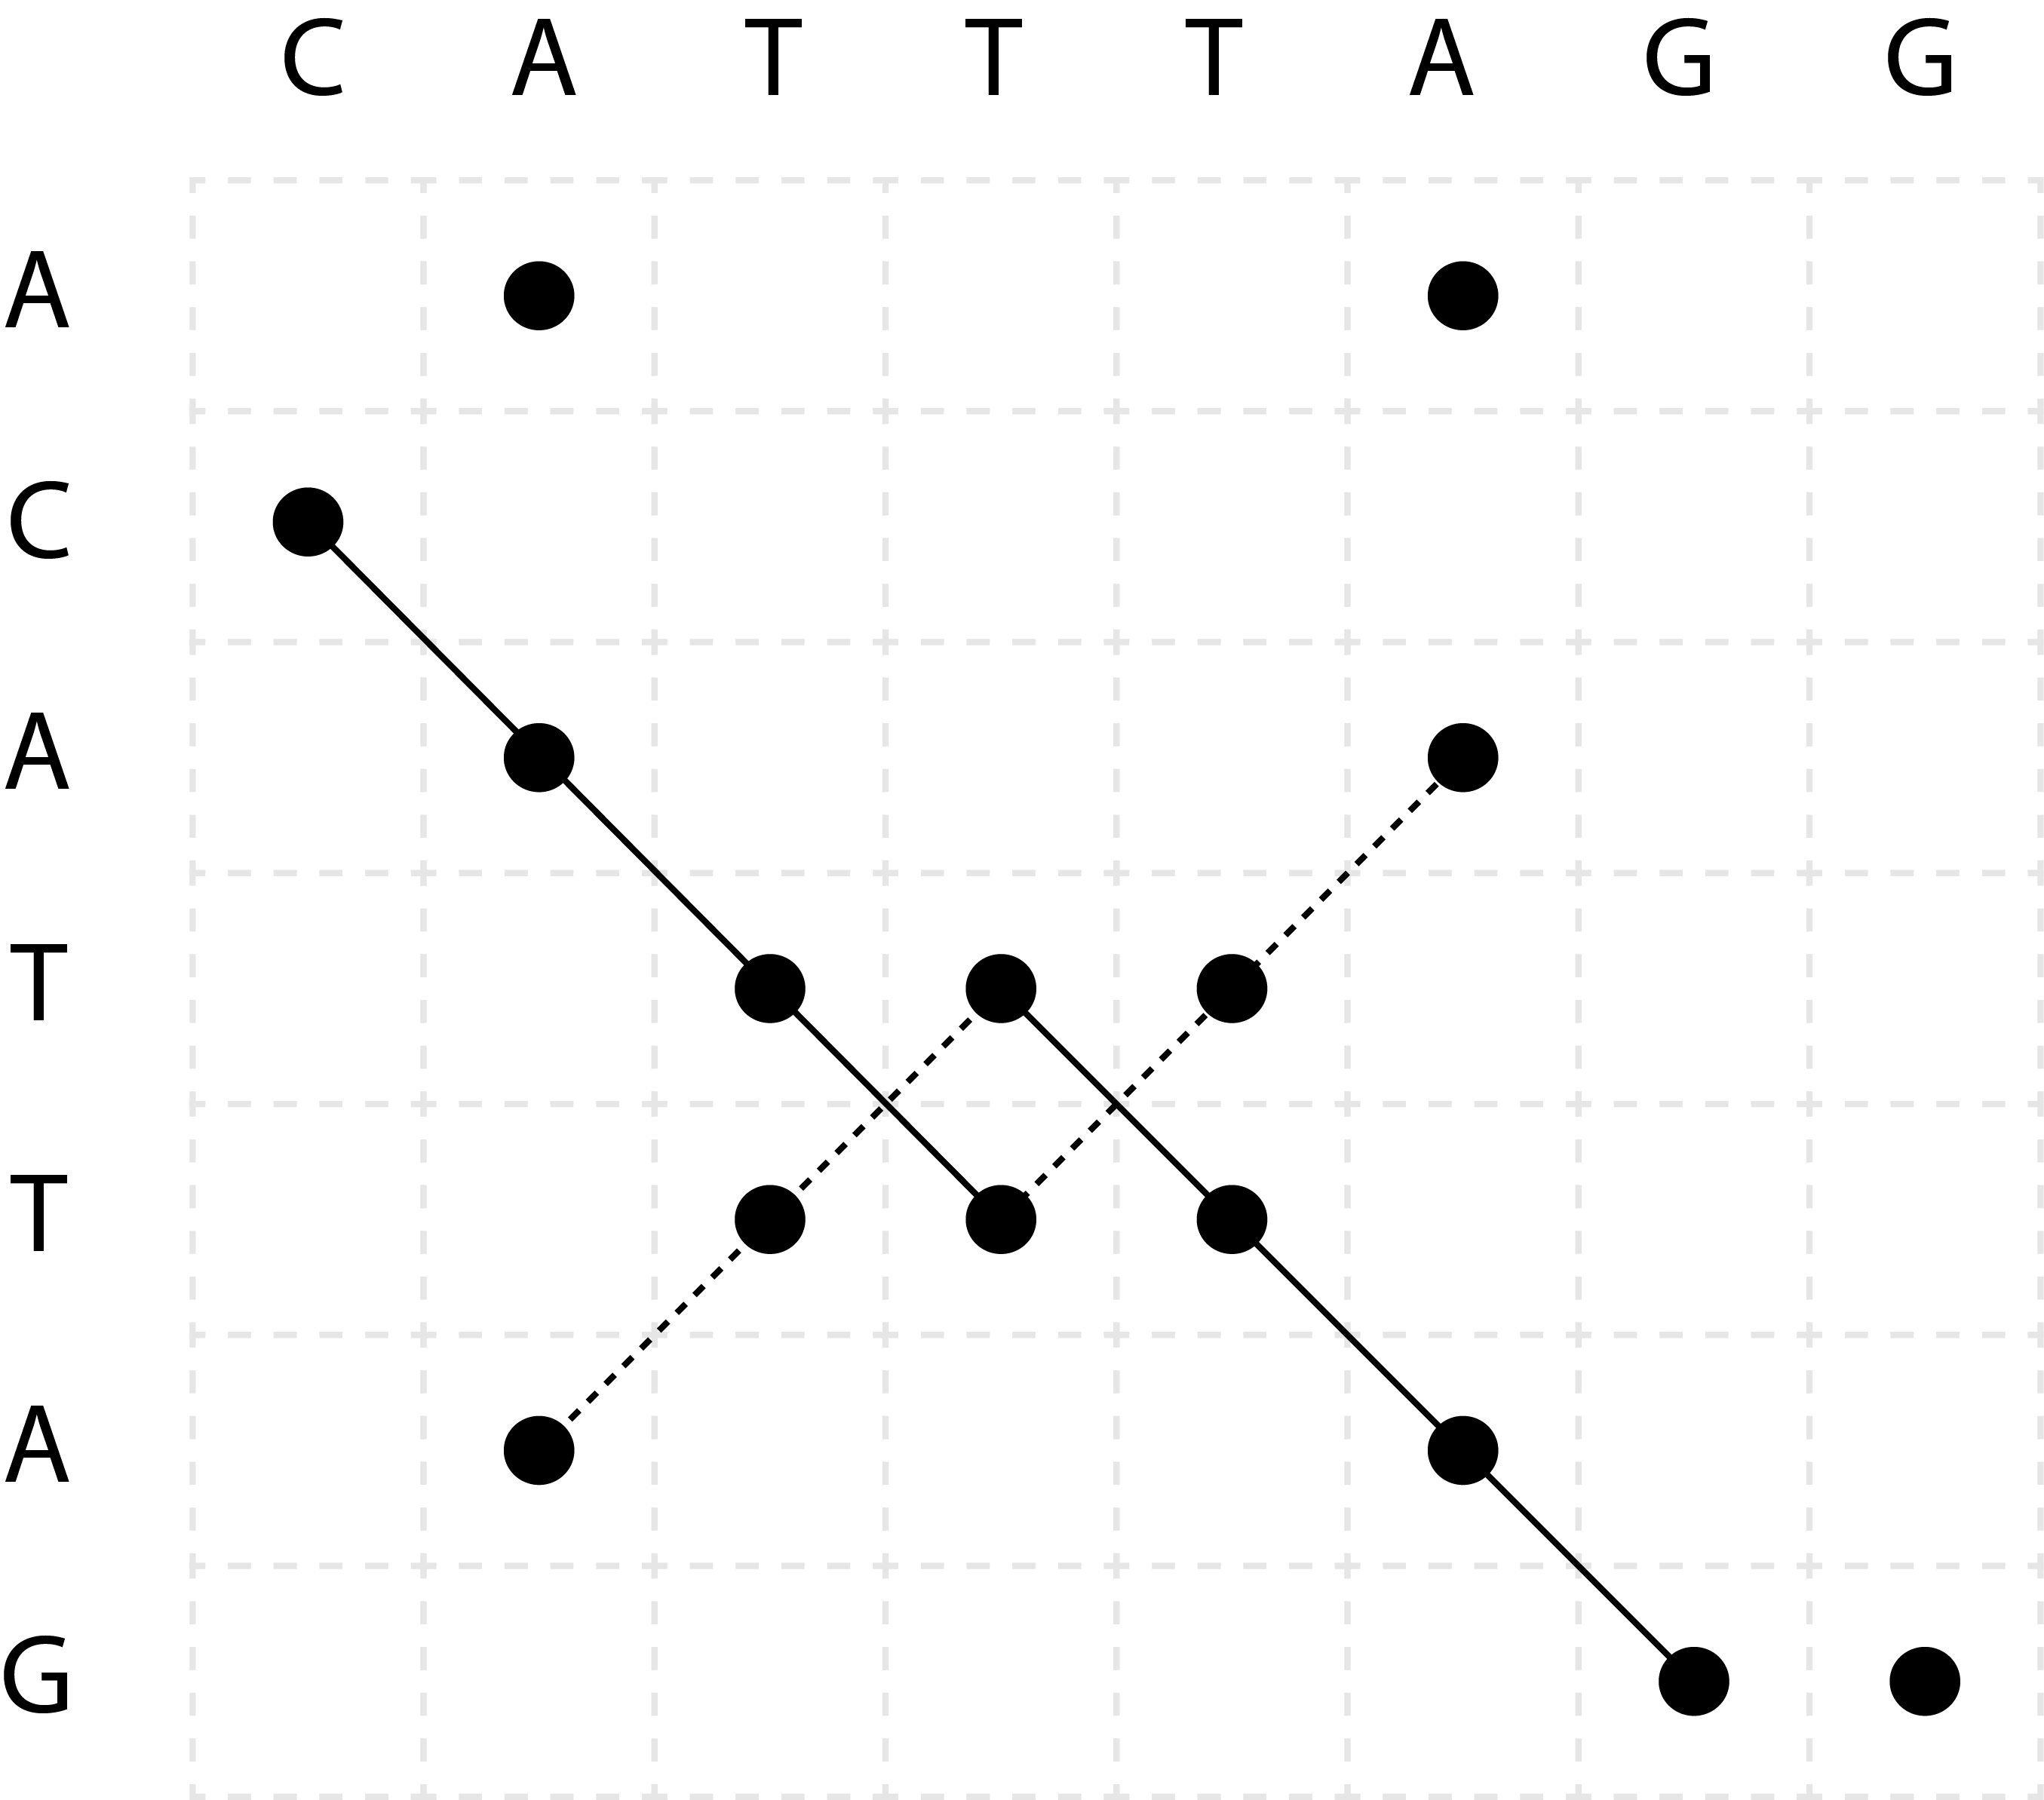
\includegraphics[width=0.3\textwidth]{fig04/dot_matrix.png}
  \caption{Filtered dot matrix with window size 3 and threshold 3.}
\end{figure}

%
% Exercise \thesection.2
%
\subsubsection*{Exercise \thesection.2}
Find local similarities between two DNA sequences, \verb|q: GATTACA| and \verb|d: GGATTTAC|.

\begin{enumerate}
\item Create a dot matrix for the two sequences.
\item Filter dots with overlapping windows size 3 and threshold 3.
\end{enumerate}

\bigskip 

%\end{document}
